\section{Angles}
\subsection{Definition of Angles}

Trigonometry is the study of angles.  An {\bf angle} is a measure of 'rotational distance'.  Take a line segment; hold one end down, and move the other.  What does the path look like?\\

The path traced by the moving endpoint is an {\bf arc}.  The formal definition of an angle is the ratio of the length of this arc to the length of its line segment, or radius.

\begin{figure}[htb]
\center
\caption{An arc and its angle.}
\label{fig:arc_and_angle}
\begin{tikzpicture}[inner sep=0pt,minimum size=0mm]
\node (r) at (1,-0.25){$r$};
\node (r) at (0.55,0.3){$\theta$};
\node (eqn) at (4,1){$\theta=\frac{l}{r} \ \ radians$};
\node () at (90:2.25){};

\LANGLE{0,0}{2.0}{0}{57.3}{$l$}

\end{tikzpicture}
\end{figure}


\subsection{Measuring Angles}

The intrinsic unit for measuring angles is the {\bf radian}.  In the previous formula, $\theta = \frac{l}{r}$, $\theta$ is in radians.  An angle of $1$ radian ($\theta = 1$) is the angle where the arc length is equal to the radius($l = r$). For a visual cue of how "big" a radian is, Figure \ref{fig:radians} shows a circle constructed from radians.  The notation for radians in an equation is 'rad' or less commonly a superscript c;  $1\  rad = 1^c = 1 \ radian$.\\

If a line segment makes a complete rotation, the resulting arc is a circle, and the angle is $2\pi$($\approx 6.28$) radians.  $\pi$($\approx 3.1415$) is the ratio of the circumference of a circle to its diameter.  This number is a constant you will see frequently.  You can see in  Figure \ref{fig:radians} that a complete circular rotation is an angle of $2\pi$ radians.\\

Because a circle represents a complete rotation, it is conventient to measure angles in fractions of a circle.  Thus, another common unit of measurement for angles is the {\bf degree}.  There are $360$ degrees in a circle.  The notation for degrees in an equation is 'deg' or a superscript o;  $1\  deg = 1^o = 1 \ degree$.\\

Since there are $2\pi$ radians in a circle, there are $\frac{360}{2\pi}$($\approx 57.3$) degrees in a radian.  Remember this!  To convert an angle from radians to degrees, multiply the radian value by $\frac{180}{\pi}$.\\

\begin{figure}[htb]
\center
\caption{Radians in a circle.}
\label{fig:radians}
\begin{tikzpicture}[inner sep=0pt,minimum size=0mm]

\node () at (90:2){};

\AXES{0}{0}{3}{3}
\LANGLE{0,0}{2.5}{0}{57.3}{$1^c$}
\LANGLE{0,0}{2.5}{57.3}{2*57.3}{$2^c$}
\LANGLE{0,0}{2.5}{2*57.3}{3*57.3}{$3^c$}
\LANGLE{0,0}{2.5}{3*57.3}{4*57.3}{$4^c$}
\LANGLE{0,0}{2.5}{4*57.3}{5*57.3}{$5^c$}
\LANGLE{0,0}{2.5}{5*57.3}{6*57.3}{$6^c$}
\LANGLE{0,0}{2.5}{6*57.3}{360}{$2\pi^c$}

\end{tikzpicture}
\end{figure}

Note that angles, by convention, are drawn as a counterclockwise rotation from the positive x axis.  An angle drawn as a clockwise rotation is considered a negative angle.\\

\begin{figure}[htb]
\center
\caption{Positive and negative angles.}
\label{fig:positive_and_negative}
\begin{tikzpicture}[inner sep=0pt,minimum size=0mm]
\node () at (90:1.25){};

\AXES{0}{0}{2.5}{2.5}
\LANGLE{0,0}{2.0}{0}{57.3}{$\theta$}
\LANGLE{0,0}{2.0}{0}{-57.3}{$-\theta$}

\end{tikzpicture}
\end{figure}

When a line undergoes a complete rotation (a rotation by $2\pi$ radians), it ends up in the same position as where it started.  A consequence of this is that for many problems, an angle $\theta$ can be replaced with an equivalent angle $\theta \pm  (2\pi)n$, where $n= 0, 1, 2...$  So, for an angle of $60^o$, $60^o + 360^o = 420^o$ or $60^o - 360^o = -300^o$ are equivalent angles.\\

\begin{figure}[htb]
\center
\caption{Equivalent angles.}
\label{fig:positive_and_negative}
\begin{tikzpicture}[inner sep=0pt,minimum size=0mm]

\AXES{0}{0}{3.25}{2.5}
\LANGLE{0,0}{2.5}{0}{60}{$60\degree$}
\SPIRAL{0}{420}{1.75}{1.25}{$420\degree$}

\end{tikzpicture}
\end{figure}

Right angles are a common sight in mathematics, and as such have a shorthand notation.  Right angles are signified by drawing a square in the corner of the angle.\\

\begin{figure}[htb]
\center
\caption{A right angle.}
\label{fig:right_angles}
\begin{tikzpicture}[inner sep=0pt,minimum size=0mm]
\node () at (0,2.25){};
\ANGLE{0,0}{2}{0}{90}

\draw (0,0.2) -- (0.2,0.2);
\draw (0.2,0) -- (0.2,0.2);

\end{tikzpicture}
\end{figure}

{\bf Complementary angles} are two angles that can be combined to form a right angle.  They do not have to be adjacent angles, just angles whose measurements add to $\pitwo$ radians.  Similarly, {\bf supplementary angles} are two angles that can be combined to form a straight angle; angles whose measurements add to $\pi$ radians.

\begin{figure}[htb]
\center
\caption{Complementary and supplementary angles.}
\label{fig:comp_and_supp}
\begin{tikzpicture}[inner sep=0pt,minimum size=0mm]
\node () at (0,2.25){};
\node () at (-3.0,-.5){complementary};
\node () at (3.0,-.5){supplementary};

\ANGLE{-3,0}{2}{0}{60}{}
\ANGLE{-3,0}{2}{60}{90}{}

\ANGLE{3,0}{2}{0}{120}{}
\ANGLE{3,0}{2}{120}{180}{}

\end{tikzpicture}
\end{figure}

\newpage

\subsection{Types of Angles}

There are several different classifications of angles: \\

A {\bf  full angle} is the angle made by a complete circle, an angle of $2\pi$ radians($360^o$). \\

A {\bf  straight angle} is the angle made by a semi-circle, an angle of $\pi$ radians($180^o$). \\

A {\bf right angle} is the angle made by a quarter-circle, an angle of $\pitwo$ radians($90^o$). \\

A {\bf reflex angle} is any angle larger than a straight angle and smaller than a full angle.  It has an angle of between $\pi$ and $2\pi$ radians(between $180^o$ and $360^o$). \\

An {\bf obtuse angle} is any angle larger than a right angle and smaller than a straight angle.  It has an angle of between $\pitwo$ and $\pi$ radians(between $90^o$ and $180^o$). \\

An {\bf acute angle} is any angle smaller than a right angle.  It has an angle of between $0$ and $\pitwo$ radians(between $0^o$ and $90^o$). \\

\begin{figure}[htb]
\center
\caption{Types of angles.}
\label{fig:types_of_angles}
\begin{tikzpicture}[inner sep=0pt,minimum size=0mm]
\node[label={[label distance=1.25cm]270:full}] (a) at (-4,3){};
\node[label={[label distance=1.25cm]270:straight}] (b) at (0,3){};
\node[label={[label distance=1.25cm]270:right}] (c) at (4,3){};
\node[label={[label distance=1.25cm]270:reflex}] (d) at (-4,0){};
\node[label={[label distance=1.25cm]270:obtuse}] (e) at (0,0){};
\node[label={[label distance=1.25cm]270:acute}] (f) at (4,0){};
\node () at (0,4.5){};

\ANGLE{a}{1}{0}{360}
\ANGLE{b}{1}{0}{180}
\ANGLE{c}{1}{0}{90}

\ANGLE{d}{1}{0}{225}
\ANGLE{e}{1}{0}{135}
\ANGLE{f}{1}{0}{60}

\end{tikzpicture}
\end{figure}


\newpage

\newpage
\subsection{Review}

\begin{enumerate}
\item {In the beginning of this chapter, I defined an angle as a measure of 'rotational distance', but I didn't state what a rotation actually is.  So, what is a rotation?  Do some research, and come up with a definition for a rotation that you find satisfactory.}

\item{What is the mathematical definition of an angle?  Write this down until you can recall it without referring back to the chapter.}

\item{What is the definition of a radian, and what is the definition of a degree?  Why would we have two different units of measure for an angle?}

\item{What is the conversion ratio for degrees to radians?  For radians to degrees?}

\item{Convert the following values in radians to degrees: \pisix, \pifour, \pithree, \pitwo, \twopithree, \threepifour, \fivepisix, $\pi$, \sevenpisix, \fivepifour, \fourpithree, \threepitwo, \fivepithree, \sevenpifour, \elevenpisix, $2\pi$.}

\item{Convert the following values in degrees to radians: 30, 45, 60, 90, 120, 135, 150, 180, 210, 225, 240, 270, 300, 315, 330, 360.}

\item{Convert the following values in radians to fractions of a circle:  \pisix, \pifour, \pithree, \pitwo, \twopithree, \threepifour, \fivepisix, $\pi$, \sevenpisix, \fivepifour, \fourpithree, \threepitwo, \fivepithree, \sevenpifour, \elevenpisix, $2\pi$.}

\item{Convert the following values from degrees to fractions of a circle: 30, 45, 60, 90, 120, 135, 150, 180, 210, 225, 240, 270, 300, 315, 330, 360.}

\item{Classify each angle as full, straight, right, reflex, obtuse, or acute:  \pisix, \pifour, \pithree, \pitwo, \twopithree, \threepifour, \fivepisix, $\pi$, \sevenpisix, \fivepifour, \fourpithree, \threepitwo, \fivepithree, \sevenpifour, \elevenpisix, $2\pi$.}

\item{Find the complement of each angle in degrees: 30, 45, 60, 90, 120, 135, 150, 180, 210, 225, 240, 270, 300, 315, 330, 360.}

\item{Find the supplement of each angle in radians:  \pisix, \pifour, \pithree, \pitwo, \twopithree, \threepifour, \fivepisix, $\pi$, \sevenpisix, \fivepifour, \fourpithree, \threepitwo, \fivepithree, \sevenpifour, \elevenpisix, $2\pi$.}

\end{enumerate}
